%-------------------------------------------------------------------------------
% seq24_song_editor
%-------------------------------------------------------------------------------
%
% \file        seq24_song_editor.tex
% \library     Documents
% \author      Chris Ahlstrom
% \date        2015-07-19
% \update      2015-07-19
% \version     $Revision$
% \license     $XPC_GPL_LICENSE$
%
%     Provides the concepts.
%
%-------------------------------------------------------------------------------

\section{Song Editor}
\label{sec:seq24_song_editor}

   The \textsl{Seq24 Song Editor} is used to combine all of the patterns
   into a complete tune.

   TODO

\begin{figure}[H]
   \centering 
   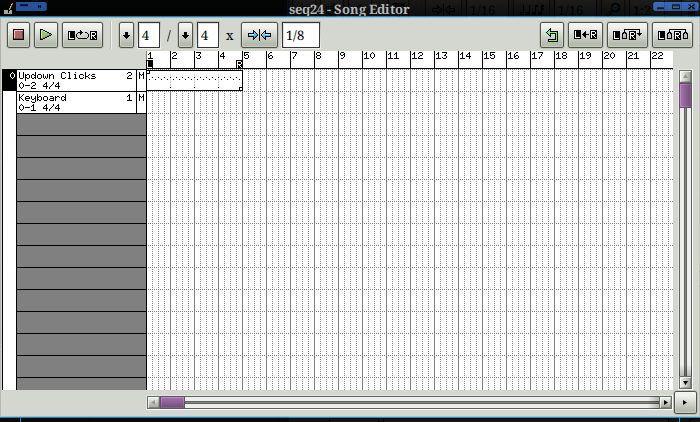
\includegraphics[scale=0.75]{song-editor/song-editor-window.png}
   \caption{Song Editor Window}
   \label{fig:song_editor_window}
\end{figure}

   This dialog is not too complex, but
   For exposition, we break it into a top panel and the rest of the window.

\subsection{Song Editor, Top Panel}
\label{subsec:seq24_song_editor_top}

   TODO

\begin{figure}[H]
   \centering 
   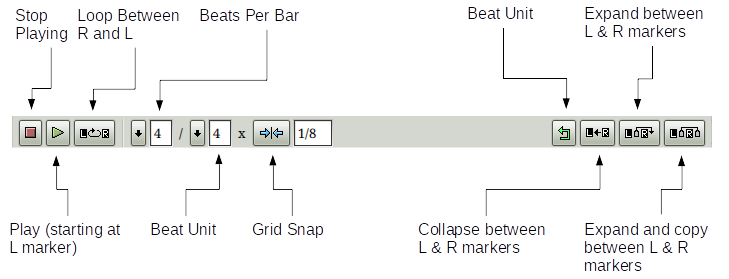
\includegraphics[scale=0.75]{song-editor/song-editor-top-panel-items.png}
   \caption{Song Editor, Top Panel Items}
   \label{fig:song_editor_top_panel_items}
\end{figure}

   TODO

\subsection{Song Editor, Arrangement Panel}
\label{subsec:seq24_song_editor_arrangement_panel}

   TODO

   See the figure at the top of this section.

   TODO


%-------------------------------------------------------------------------------
% vim: ts=3 sw=3 et ft=tex
%-------------------------------------------------------------------------------
